\chapter{Introduction}
\label{ch:chap1}


%------------------------------------------
\section{Background}

\subsection{Engineering Background}

Peripheral artery disease (PAD) is a narrowing of arteries along legs. It is a major cause of amputation in United States \cite{conte2016critical}. It is prevalent among smokers, diabetics and patients with dyslipidemia. Meanwhile, the long waiting time and expensive cost are two major problems that affect patients. In the modern clinic, doctors are actively looking for a solution which can provides both high fidelity and high resolution images to analyze the PAD. The  present CT scan technology can only render a two-dimensional,  monochrome, static and low-resolution pictures. In recent decades, many researchers have contributed numerous efforts on improving the diagnosis of stenoses and the quality of images \cite{clark1976fluid, nesbitt2009shear, wardlaw2006non, stergiopulos1992computer, long2001numerical}. With the fast development of both hardware and computing algorithms, the computational simulations are aiming to provide 3D, dynamic, high resolution and patient-specific results.

\begin{figure}[H]
	\centering
	\begin{tabular}{c}
		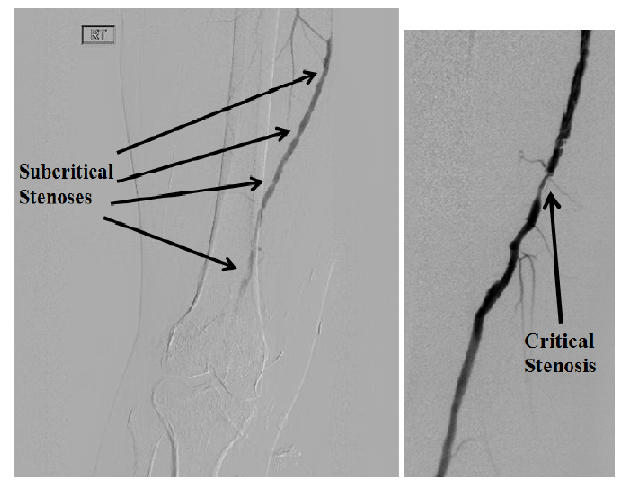
\includegraphics[width=0.6\textwidth]{./pics/photo.png}
	\end{tabular}
	\caption{\footnotesize Critical stenosis and subcritical stenoses.} \label{fig: photo}
\end{figure}

Fig. \ref{fig: photo} is the CT scan image. It shows the difference between single critical stenosis and multiple subcritical stenosis. Currently, doctors employ stent to treat the critical stenosis. However, the impact of multiple subcritical stenoses is unclear yet. Computational simulation is a great tool to assist doctors to evaluate and make decision.
Compared to current CT scans, it is significantly faster, less expensive and more accurate. In addition, it is also very important that the simulation results provide the dynamic growth animations of current stenoses and the developing path after the clinic treatment to doctors and patients. 

\begin{figure}[H]
	\centering
	\begin{tabular}{c}
		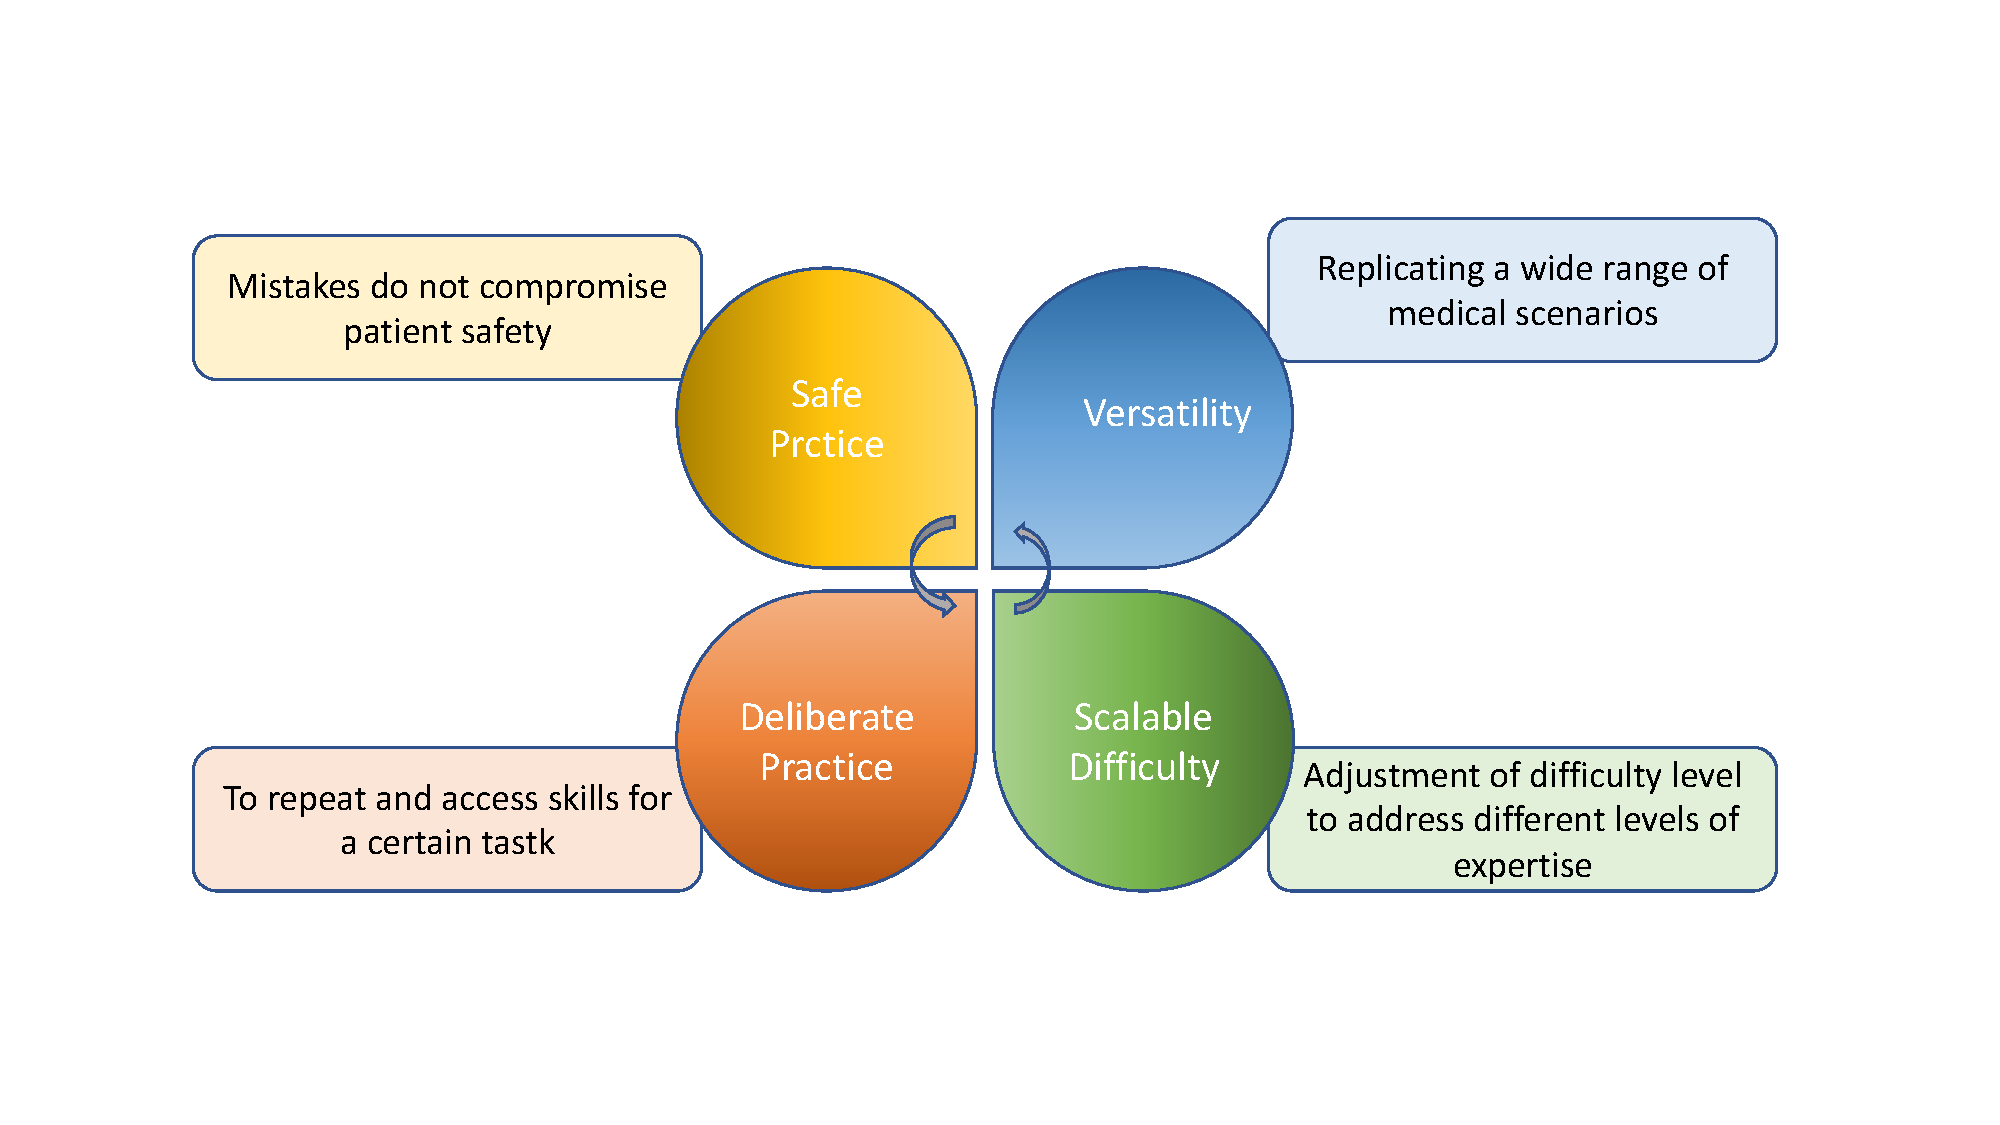
\includegraphics[width=1.0\textwidth]{./pics/computer_simulation}
	\end{tabular}
	\caption{\footnotesize Different factors affecting computer-based medical simulation.} \label{fig: ch1f1}
\end{figure}

Fig \ref{fig: ch1f1} summarizes some factors which contribute to the related components in computational medical simulation technology \cite{barry2005features}. Many investigations have been conducted through last decades \cite{feng2012viscous, bertram2010evaluation, nadeem2010simulation, ogulu2005simulation}. We are interested in investigating the impact comparison between single critical stenosis with multiple sequential subcritical stenoses. We aims to discover the high fidelity simulation results of comparison between single critical stenosis with multiple subcritical stenoses along peripheral artery.

In Fig \ref{fig: ch1f1}, it shows the factors affecting the computational simulation applying on PAD study. Safe practice refers to contact-less and safety; Versatility refers to the flexibility to construct patient specific case; Deliberate practice refers to the accuracy of diagnosis from doctors and scalability difficulty refers to the learning curve for doctors to employ.

Physically, the PAD can be abstracted as a fluid-structural interaction (FSI) problem by using fluid and structural dynamics equations, respectively.  There are two approaches for solving such FSI problems, the monolithic method \cite{hubner2004monolithic, degroote2009performance} and the partitioned method \cite{kuttler2008fixed, vierendeels2007implicit}. For the monolithic method, the two sets of equations are solved in one large linear system simultaneously. This mutual influence can be considered as internal forces. One significant advantage of this scheme is simplicity. Only a single global matrix is constructed so that both the fluid and structural parts can be solved under the same spatial discretization and time marching scheme. For the trade-off, we loose the flexibility to control fluid and structural parts individually. The other approach is the partitioned method. The two sets of equations are solved separately by passing results as boundary conditions to each other. The solution of fluid equations is calculated while the structural part waits for new boundary condition input, and vice versa. The partitioned method requires a coupling algorithm to exchange the interaction between the two phases as a pair of modules. The Implicit-Explicit (IMEX) Runge-Kutta (RK) time integration approach has been illustrated to be accurate and efficient \cite{zhang2016high}.

A Finite-Volume fluid solver \cite{liang2007large, liang2007large1, liang2009effect} is accomplished and a series of CFD studies has been implemented on idealized geometries. To implement a more high-fidelity simulation, the tissue of blood vessel wall shall be considered as elastic material. Therefore, an accurate and efficient structural solver for solving the elasticity equation is needed. The solver should be capable of calculating the material behavior according to the stiffness property, which is the response of the deformable model reacting to the external forces. The simplest model is a mass-spring model, which is easy to compute but can not accurately determine the details of material behavior. A more precise approach is the finite element method (FEM), which is based on the continuum mechanics, is more popular. The FEM can specify the stiffness of the model by only using a few characteristic parameters, such as Young's modulus, Poisson ratio and the geometries. However, the challenge for 3D FEM simulation is its parallelization in large-scale parallel computational fluid-structure interaction frameworks is to be used in real-time application due to the very expensive computational cost. 

\begin{figure}[H]
	\centering
	\begin{tabular}{c}
		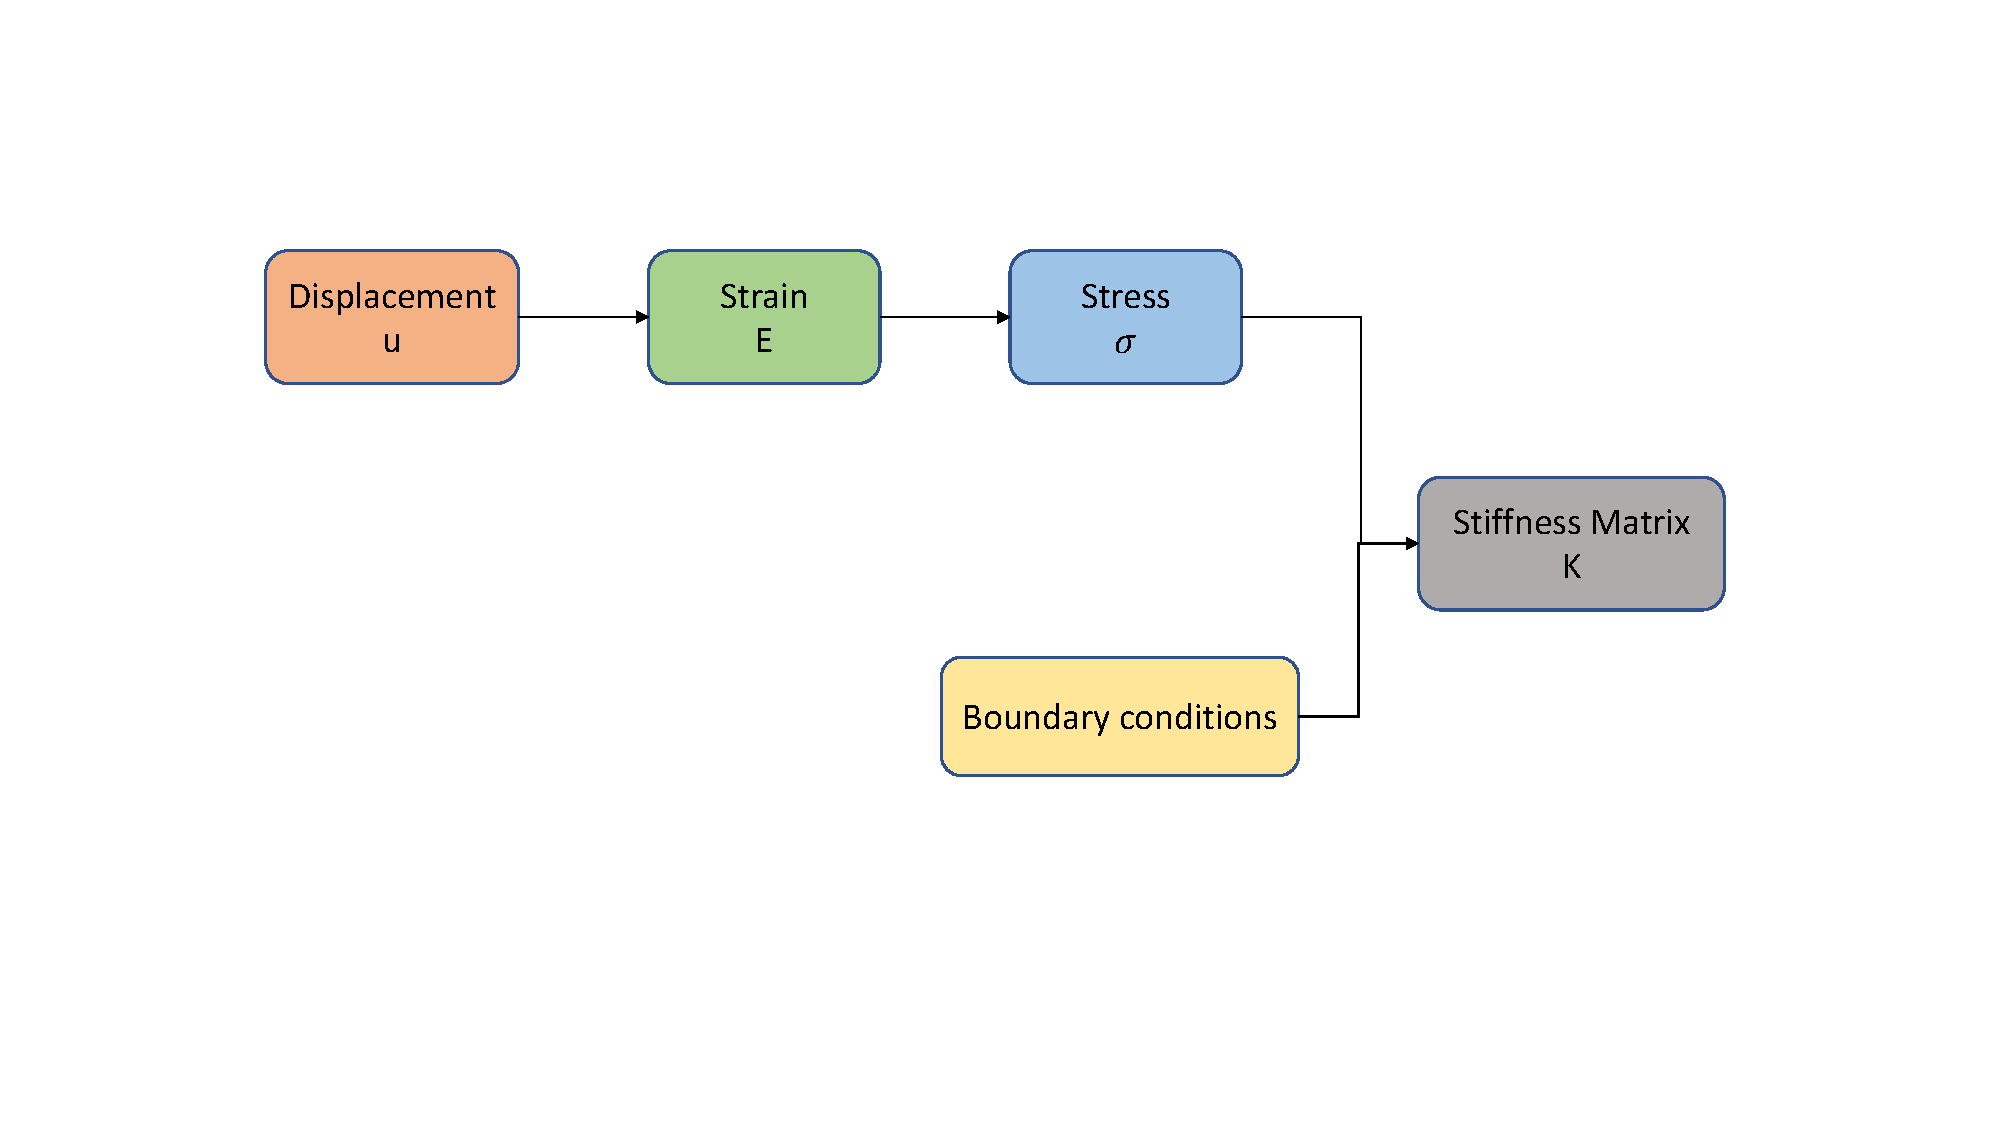
\includegraphics[trim = 40mm 25mm 0mm 10mm,clip,width=1.2\textwidth]{./pics/construct_matrix}
	\end{tabular}
	\caption{\footnotesize Construct stiffness matrix.} \label{fig: ch1f2}
\end{figure}

Fig \ref{fig: ch1f2} shows a general process of calculating a deformable material object. Applying stress-strain relation, the unknown variable of governing equation is converted to strain tensor $ \varepsilon $. Then after applying the strain-displacement relation, the unknown variable is displacement vector $ u $. The FEM employs basis function to convert the continuous function into construct the discrete matrix $ K $. Combine with the boundary condition $ \hat{u} $ and loading force $ f $, we can solve the linear system and obtain the solution.

\begin{figure}[H]
	\centering
	\begin{tabular}{c}
		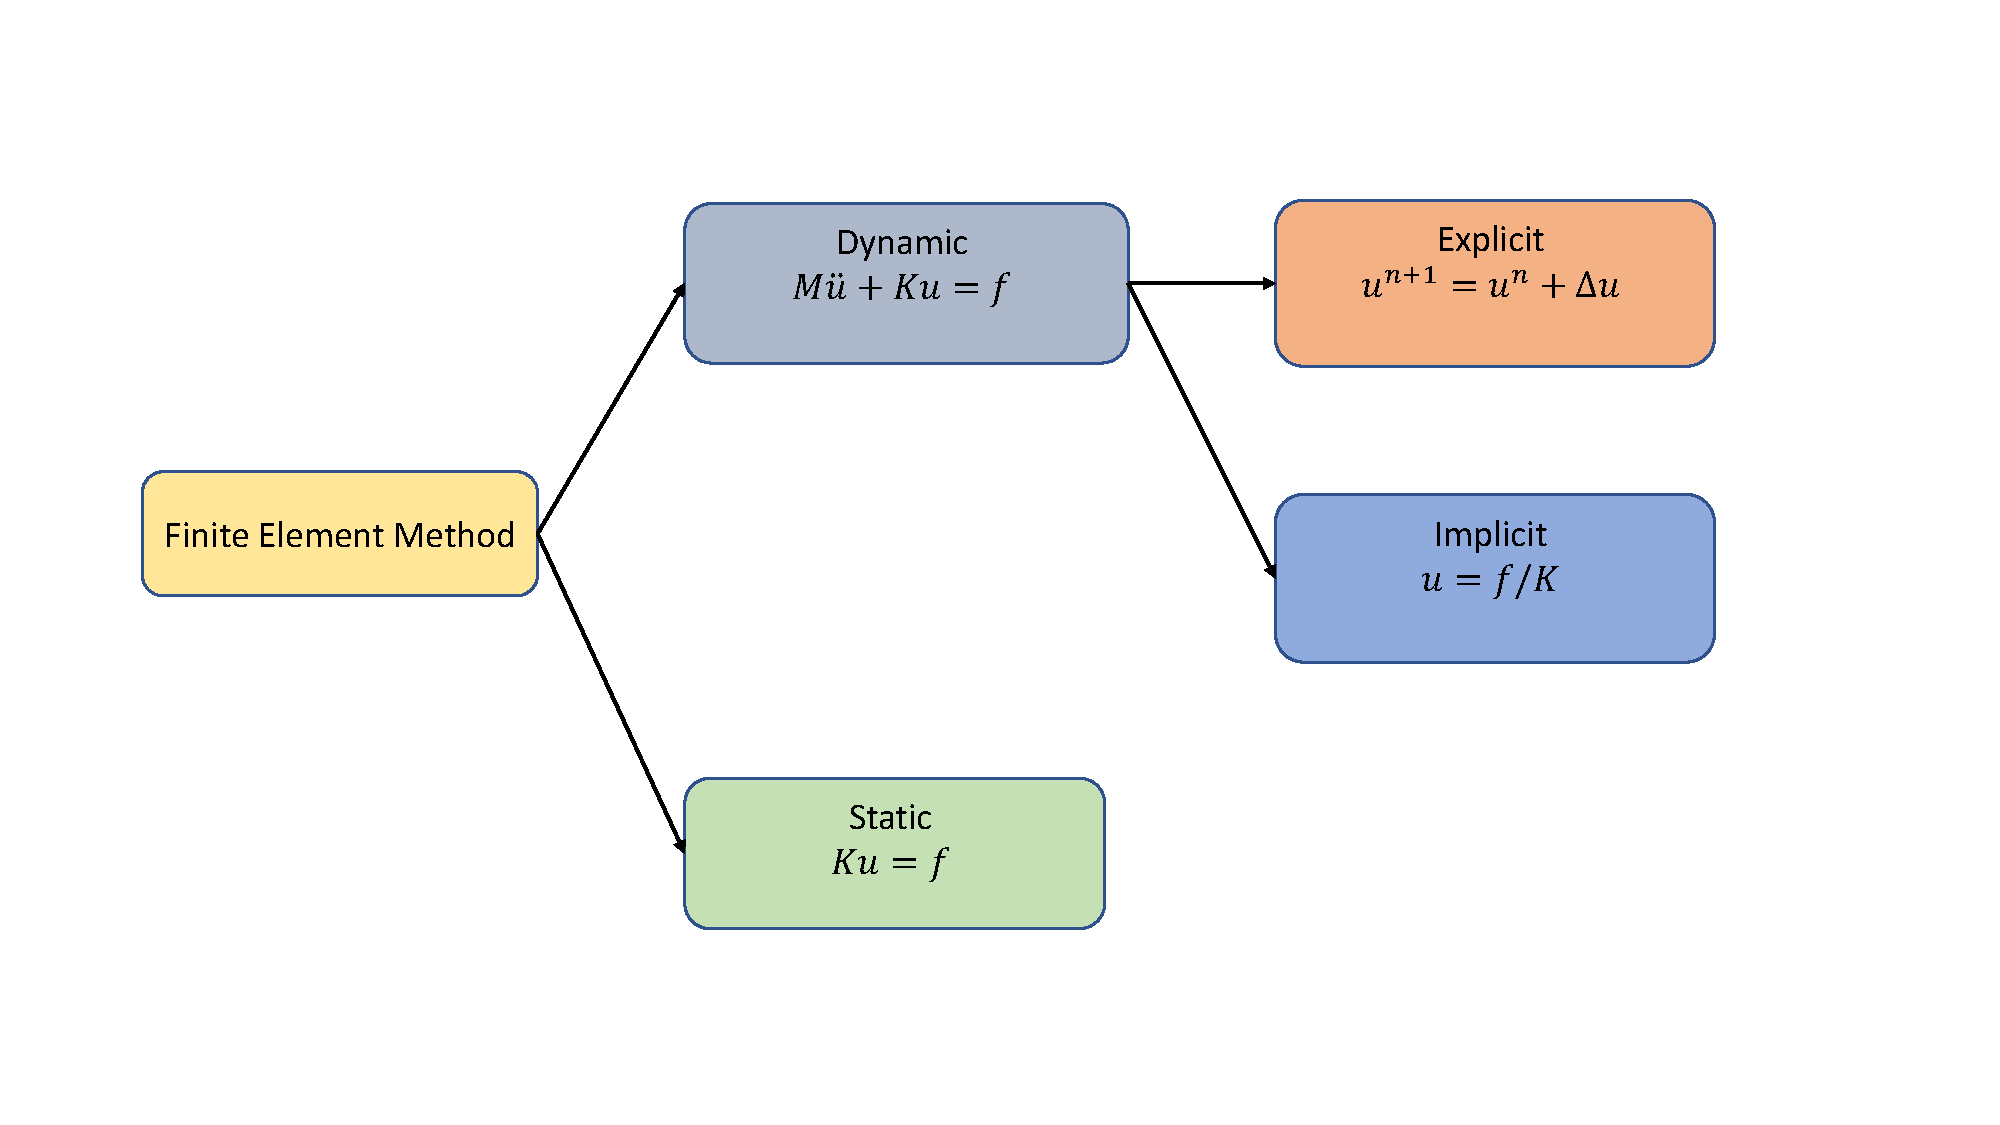
\includegraphics[width=1.1\textwidth]{./pics/fem}
	\end{tabular}
	\caption{\footnotesize Static and dynamic finite element method.} \label{fig: ch1f3}
\end{figure}

The Fig \ref{fig: ch1f3} displays both static analysis and dynamic analysis for elasticity equations. The steady-state and transient finite element problem are studied with static analysis and dynamic analysis, respectively. The latter one is time dependent. In dynamic analysis, we shall consider the spatial discretization by using both explicit and implicit time marching schemes \cite{bathe2008finite}. The implicit time marching scheme is computational costly, because a matrix inversion for large linear system is required every time-step. The benefit is unconditionally stable for large time steps. On the other hand, the explicit time marching scheme requires less computational cost for each time-step. However, the size of each time step has to satisfy the numerical stability criteria. 


Commonly, the linear system of elasticity equations derived from the FEM method is positive definite . For real engineering problem, the size is too large to be directly computed. The most time consuming part in the FEM analysis in Fig \ref{fig: ch1f2} is solving the linear system. The complex system can be written in a matrix form $ \mathbf{A} \mathbf{x} = \mathbf{b} $. To solve it, there are two approaches: the direct method and the iterative method. Considering the better performance on memory usage and shorter computing time, the iterative method is preferred for large scale problems \cite{brussino1989comparison}. The Preconditioned Conjugate Gradient (PCG) is one of the most popular methods because of its robustness and fast convergence rate. However, the PCG requires positive definite matrices. It is still very challenging to implement finite element analysis using an implicit scheme to study the material real-time response behavior due to the excessive computational cost. Therefore, the domain decomposition method combined with a parallel computing scheme is one emerging choice to reduce computational cost.

Parallel computing desires optimal load balance to achieve high concurrent execution in terms of computational time. The challenges to reach that purpose include learning and understanding programming paradigms,  balancing the loads to maximize the usage of bandwidth, minimizing the overhead on data communication and avoiding potential data racing problems. To achieve a good level of parallelism, we employ some modern techniques such as MPI, Intel Math-Kernel library and LAPACK-BLAS for optimal scalability by reducing the overhead latency with a large number of active processors and ensure the balance of loads on each processor.

\subsection{Overview of Related Numerical Methods}

The Weak Galerkin Finite Element Method (WG-FEM) is an efficient numerical method for solving partial differential equations. The WG method is recently developed by Dr. Junping Wang and Dr. Xiu Ye in 2011 and applied for solving second order elliptic equations\cite{wang2014weak}. The WG method introduces a series of weak operators such as weak gradient, weak divergence and weak curl operators for the computation of corresponding strong forms of differential equations. The WG finite element method provides a  new perspective to solve numerical problems. The WG method can be applied on a variety of partial differential equations, such as second order elliptic equation, elasticity equation\cite{wang2016locking}, Stokes equations \cite{wang2016weak} and Maxwell's equations \cite{mu2013weak}, etc. The WG method is a discontinuous method. It has two distinct components, weak gradient function and stabilizer. We defined weak function which divides an element into interior and boundary space. Different order of polynomials can be applied on two spaces independently. The weak gradient function connects the unknown variables and weak gradient operator and constructs the elemental matrix. The stabilizer connect the interior and boundary space in a form of boundary integral of projected value difference. The details of the WG method will be discussed in Chapter 2.

%-----------------------------------------------------
\section{Objectives}

The objective of this dissertation is to develop an efficient parallel structure solver by using WG method on unstructured meshes. We deliver it in two steps: designing an improved stabilizer for time marching scheme and developing the WG-BDDC method to solve elasticity problems. The stabilizer is designed for completing mass matrix to enable dynamic study. The WG-BDDC is the first attempt to bring the WG method in the engineering filed and implement it on parallel computers. 

The classic continuous Galerkin (CG) finite element analysis of continuum mechanics is widely used to study and predict material deformations. The results are generally accurate and reliable for analyzing the relationship between load and deformation. However, the computational complexity prevents wide adoption to solve large-scale FSI problems. Massively parallel computing is required for obtaining large linear system. In this work, we develop efficient parallel schemes, which is capable for solving large scale elasticity equation.

We employ the WG-FEM to convert the bilinear form equations into a positive definite linear system. The WG method can use multiple types of elements. The selection of polynomials on interior or boundary region is flexible which enhances the freedom of computational simulation for dealing with complex geometries. Moreover, the discontinuous features in the WG method facilitates the implementations of parallel computations.

The Balancing Domain Decomposition by Constraints (BDDC) method is a new approach for the WG-FEM to achieve parallelism on distributed-memory computers. BDDC identifies the two spaces (primal and dual) and applies the divide and conquer strategy (Block Cholesky) to the original computational domain. By minimizing the global communication and synchronization overhead,  WG-BDDC can effectively solve equations with superlinear scalability on parallel computers.

 Fig \ref{fig: ch1p4} shows the paths to accomplish the objectives in this work. This research aims to significantly improve the computational efficiency of the elastic material response, including in clinic judgment and other medical applications.

\begin{figure}[H]
	\centering
	\begin{tabular}{c}
		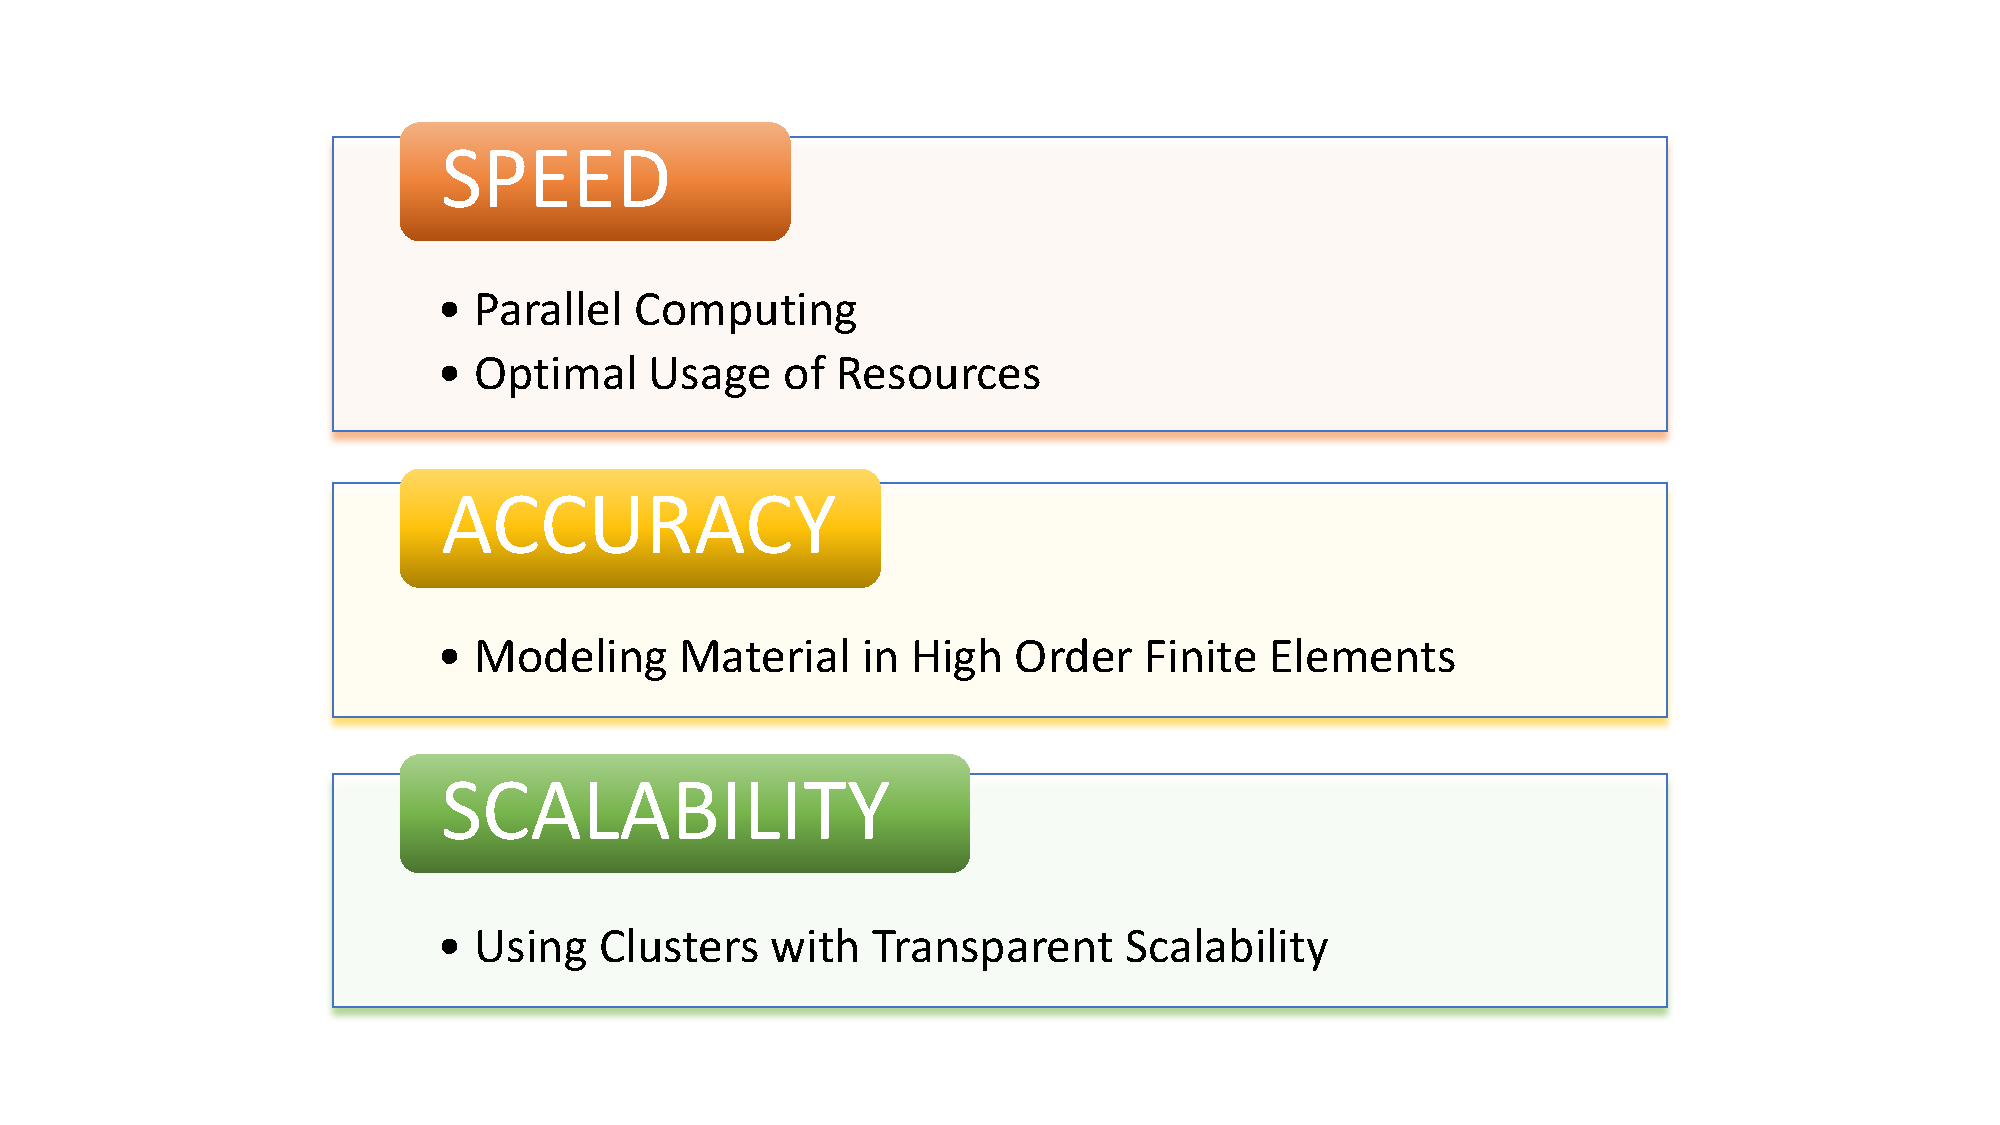
\includegraphics[width=1.0\textwidth]{./pics/ch1p4}
	\end{tabular}
	\caption{\footnotesize Objectives and methodology.} \label{fig: ch1p4}
\end{figure}

To validate the WG-BDDC scheme and develop a powerful software, we first design a hybrid WG-CG element. The results are consistent with the benchmark of serial CG solver. Then, we extend the WG elements to integrate with BDDC method and verify the convergence and the order of accuracy of the new method (WG-BDDC) on parallel computers. Finally, the scalability is discussed under the parallel computing framework.

The rest of this dissertation is organized as :

\begin{itemize}
	\item Chapter 2 presents the background and basics of the WG method.
	\item Chapter 3 discusses the hybrid WG-CG finite element method. We also tested the performance of the hybrid method for nonlinear elasticity equation.
	\item Chapter 4 introduces the WG-BDDC method for second order elliptic and elasticity equation.
	\item Chapter 5 concludes this work and directions for future works.
%	\item Appendix A summarizes my study of the effect of multiple sequential stenoses on peripheral artery disease.
\end{itemize}
